\documentclass[12pt]{article}

\usepackage{fullpage,soul,graphicx,esvect,changepage,stoversymb}
%                              ^ for underline: \ul{...}
\everymath{\displaystyle}
%\pagenumbering{gobble}

\usepackage{multicol}
\usepackage[many]{tcolorbox}
\usepackage{tikz}
\usepackage{booktabs}
\usepackage[inline]{enumitem}
\usepackage{pgfplots}


\usepackage[letterpaper, margin=0.375in, top=0.5in, bottom=0.75in]{geometry}

%\setenumerate{itemsep=0.25in}
\setlist[enumerate,1]{leftmargin=0.2in, itemsep=0.625in, topsep=4.5mm}
\setlist[enumerate,2]{label=(\alph*),leftmargin=0.5in, itemsep=1in, topsep=0in}

\graphicspath{ {./../img/} }
\DeclareGraphicsExtensions{.pdf}

\newcommand{\scratch}{\newpage\thispagestyle{empty}\begin{center}Scratch Paper\end{center}}
\newcommand{\sol}{\par\vspace{4.5mm}\hspace{-4.5mm}\textsc{Solution:}}
\newcommand{\hint}[1]{\quad\textbf{Hint}: #1}
\newcommand{\note}[1]{\textbf{Note}: #1}
\newcommand{\pts}[1]{(\textit{#1 pts})}
\newcommand{\ptss}[1]{(\textit{#1 pt})}
\newcommand{\ptsea}[1]{(\textit{#1 pts ea.})}
\newcommand{\ptssea}[1]{(\textit{#1 pt ea.})}
\newcommand{\axes}[1]{\begin{center}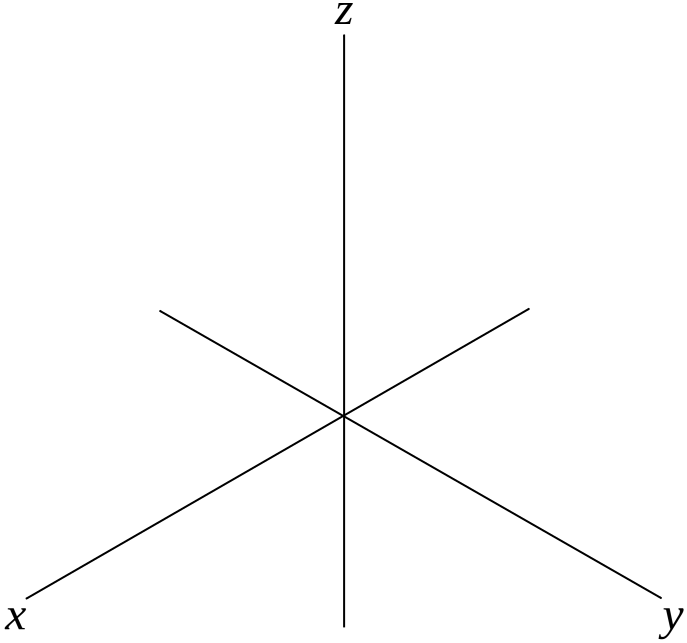
\includegraphics[scale=#1]{3DAxes}\end{center}}
\newcommand{\axespt}[1]{\begin{center}\includegraphics[scale=#1]{3DAxesWithPoint}\end{center}}
\newcommand{\pic}[2]{\begin{center}\includegraphics[scale=#1]{#2}\end{center}}
\newcommand{\comps}[1]{\langle #1_1,#1_2,#1_3\rangle}
\newcommand{\compslong}[3]{\langle #1, #2, #3\rangle}

\begin{document}
	\begin{flushright}
		{\large \textbf{Homework 4}}{\textbf{\scriptsize{/test prep 1}}}\hfill Name: \line(1,0){200}\\
		{\mbox{\hspace{1.75mm}}\small(front and back)}\hfill{\small (please print neatly!)}\mbox{\hspace{0.7in}}
	\end{flushright}
	\vspace{-1.5mm}
	\begin{adjustwidth}{0.5in}{0.5in}
		\begin{tcolorbox}[
			arc=0pt, colback=white, colframe=black, boxrule=0.5pt, before upper={\parindent15pt \parskip=3mm}]
			
			{\noindent\textbf{Directions:} Answer each of the following \textbf{\ul{three} (3)} questions, making sure to read the instructions for \ul{each question} as you proceed. \ul{If you use the Laplace table, make sure you specify which entry/entries you're referencing!}\par
			
			\textbf{Make sure that your submission meets the criteria of the \ul{Homework Policy} on the \texttt{Homework} tab of the course webpage!}\par
			
%			\begin{center}\fbox{\,\textbf{Note:} Questions 1--3 are good quiz prep; all are good exam prep!\,}\end{center}
		
			\hfill\textbf{Due date:} Monday, July 31}
		\end{tcolorbox}
	\end{adjustwidth}
		
	\begin{enumerate}
		\item Find the Laplace transform of each of the following functions.
		\begin{enumerate}
			\item $f(t)=e^{3t}\sin(4t)$
			\item $f(t)=e^{3t}\sin(4t)+e^{3t}\cos(4t)$
			\item $f(t)=e^{3t}\sin(4t)\cos(4t)$ \hint{Use a double-angle formula.}
			\item $f(t)=\left\{\begin{array}{rcl}4.913 & \text{if} & 0\leq t<2\\ e^{3t}\sin{4t} & \text{if} & 2\leq t<5\\ 2-t & \text{if} & 5\leq t<14\\ t^2 & \text{if} & t\geq 14 \end{array}\right.$
			\item $f(t)=te^t\sin{t}$. \hint{Let $g(t)=t\sin{t}$ and rewrite $f(t)$ as $f(t)=e^{ct}g(t)$ for some constant $c$.}
		\end{enumerate}
		
		\newpage
		
		\item Use partial fractions to find the inverse Laplace transform of each of the following functions $F(s)$, i.e. find the function $f(t)$ for which $\lamL\{f(t)\}=F(s)$.
		\begin{enumerate}
			\item $F(s)=\frac{1}{s^4}$
			\item $F(s)=\frac{s}{(s+1)(s-1)}$
			\item $F(s)=\frac{1}{s^2(s+1)^2(s^2+1)^2}$ \vspace{3mm}
			
			\hint{The denominator consists of repeated factors; brush up on how to handle those!}
			\item $F(s)=\frac{8s^2-4s+12}{s^2(s+1)(s^2+9)}$
			\item $F(s)=1$ \vspace{3mm}
			
			\hint{You don't know this function (err...``function''), but...tell me something about what would need to happen to make this true! Try guessing and checking some stuff, etc. etc. Think like a mathematician!}
			
			\item $F(s)=\frac{s^2}{(s+1)(s-1)}$\vspace{3mm}
			
			\hint{Let $\delta(t)$ denote the function from (e) [which you don't know] and use long division!}
		\end{enumerate}
		
		\item Solve each of the following IVPs using Laplace transforms; then, check your answers using characteristic equations and/or undetermined coefficients. \textbf{Do not check using variation of parameters!}
		\begin{enumerate}[itemsep=1.1in]
			\item $y''-5y'+6y=0$, $y(0)=0$, $y'(0)=1$
			\item $y''+4y=0$, $y(0)=1$, $y'(0)=3$
			\item $y''-5y'+6y=\frac{t^3}{3!}$, $y(0)=1$, $y'(0)=1$ \hint{Recall: $n!=n(n-1)(n-2)\cdots3\cdot2\cdot1$}
			\item $y''+4y'+4y=e^t+t$, $y(0)=-2$, $y'(0)=-2$
			\item $y''-8y'-9y=\cos{t}-\sin(2t)$, $y(0)=0$, $y'(0)=-1$
			\item $y''+4y=\cos{t}-\sin(2t)$, $y(0)=2$, $y'(0)=-1$
			\item $y''-4y=te^{-3t}\cos{t}-\sin(2t)$, $y(0)=4$, $y'(0)=0$ \hint{See 1(e) for how to handle $te^{-3t}\cos{t}$.}
		\end{enumerate} 
		
	\end{enumerate}
\end{document}